\documentclass[conference]{IEEEtran}

\usepackage{cite}
\usepackage{amsmath,amssymb,amsfonts}
\usepackage{graphicx}
\usepackage{textcomp}
\usepackage{booktabs}
\usepackage{multirow}
\usepackage{url}
\usepackage{xcolor}
\usepackage[T1]{fontenc}

\graphicspath{{figures/}}

\begin{document}

\title{Lightweight Distilled CNN for Zak-OTFS Channel Estimation: An Accuracy-Efficiency Tradeoff Study}

\author{
\IEEEauthorblockN{Author A\IEEEauthorrefmark{1},
Author B\IEEEauthorrefmark{1}}
\IEEEauthorblockA{\IEEEauthorrefmark{1}Department of Electrical Engineering\\
University Placeholder, City, Country\\
\{authora, authorb\}@university.edu}
}

\maketitle

% ══════════════════════════════════════════════════════════════
\begin{abstract}
Zak-OTFS with superimposed spread pilots has recently been proposed as a robust framework for delay-Doppler (DD) domain channel estimation in high-mobility scenarios. The associated CNN-aided estimator significantly outperforms conventional read-off methods but incurs non-trivial computational cost due to its 245k-parameter architecture. In this work, we investigate knowledge distillation as a principled approach to compress the CNN estimator while preserving estimation quality. We design a family of lightweight student architectures (Lite-L, Lite-M, Lite-S) and train them via a weighted combination of teacher-imitation and ground-truth losses. Experimental results on a Vehicular-A channel with fractional delay-Doppler show that the proposed Lite-M model, with only 22,789 parameters (a 10.8$\times$ reduction), achieves NMSE within 0.9\,dB of the teacher and comparable BER at moderate pilot-to-data ratios, while providing a measured 1.9$\times$ inference speedup. Performance gaps widen at challenging operating points, as expected under aggressive compression. The extreme-compression Lite-S variant (6,137 parameters, 40$\times$ reduction) exhibits more visible degradation but still substantially outperforms the conventional estimator. The accompanying codebase, including a reproducible baseline reimplementation, will be released to support further research.
\end{abstract}

\begin{IEEEkeywords}
Zak-OTFS, channel estimation, knowledge distillation, model compression, delay-Doppler, CNN
\end{IEEEkeywords}

% ══════════════════════════════════════════════════════════════
\section{Introduction}
\label{sec:intro}

Orthogonal time frequency space (OTFS) modulation and its principled Zak-transform formulation offer natural resilience to time-varying channels by operating in the delay-Doppler (DD) domain~\cite{hadani2017otfs, mohammed2021ddzc}. The Zak-OTFS framework with superimposed spread pilots~\cite{zakotfs2024} enables joint pilot and data transmission without guard-band overhead, while a CNN is reported to refine the conventional cross-ambiguity-based channel estimate to performance approaching the perfect-CSI bound.

However, the baseline CNN architecture uses large convolutional kernels (up to $27 \times 27$) and 245,473 trainable parameters. While this is modest by modern deep learning standards, it may be excessive for latency-sensitive or resource-constrained deployment scenarios such as vehicular edge devices. Model compression via knowledge distillation~\cite{hinton2015distilling, gou2021kd_survey} offers a natural path to reduce computational cost while retaining the estimation quality learned by the teacher.

In this paper, we make the following contributions:
\begin{enumerate}
    \item We provide a reproducible reimplementation of the Zak-OTFS superimposed spread pilot system and CNN-aided estimator, since no official code accompanies the original publication~\cite{zakotfs2024}.
    \item We design a family of compact student CNN architectures (Lite-L, Lite-M, Lite-S) that preserve the teacher's real/imaginary split processing pattern while significantly reducing parameter counts and kernel sizes.
    \item We train students via a combined distillation loss that balances teacher imitation and ground-truth regression, and we systematically evaluate the accuracy-efficiency tradeoff across NMSE, BER, parameter count, and inference latency.
\end{enumerate}

The remainder of this paper is organized as follows. Section~\ref{sec:related} reviews related work. Section~\ref{sec:system} summarizes the Zak-OTFS system model. Section~\ref{sec:baseline} describes our baseline reimplementation. Section~\ref{sec:distill} presents the proposed distillation method. Sections~\ref{sec:setup} and~\ref{sec:results} detail the experimental setup and results. Section~\ref{sec:complexity} provides the complexity analysis, and Section~\ref{sec:conclusion} concludes.

% ══════════════════════════════════════════════════════════════
\section{Related Work}
\label{sec:related}

\textbf{OTFS channel estimation.}
Early OTFS systems use embedded pilot symbols in the DD grid with surrounding guard bands, requiring dedicated overhead that reduces spectral efficiency~\cite{raviteja2019otfs}. The Zak-OTFS formulation replaces embedded pilots with superimposed spread pilots that exploit the self-ambiguity lattice structure for interference-free channel read-off on a twisted support set, eliminating guard-band overhead entirely~\cite{zakotfs2024}. Deep learning approaches for DD-domain channel estimation have been explored in~\cite{srivastava2023dnn_ce, li2022dd_channel}, though these typically target different pilot configurations.

\textbf{Knowledge distillation.}
Knowledge distillation~\cite{hinton2015distilling, buciluamodel2006} trains a compact student network to mimic a larger teacher. FitNets~\cite{romero2014fitnets} extended this to intermediate representations. Surveys such as~\cite{gou2021kd_survey} categorize approaches into response-based, feature-based, and relation-based distillation. Our approach uses response-based distillation (matching teacher outputs) combined with a ground-truth loss term, which provides a simple yet effective training signal for regression tasks.

% ══════════════════════════════════════════════════════════════
\section{System Model and Background}
\label{sec:system}

We briefly summarize the Zak-OTFS system from~\cite{zakotfs2024}. The system operates on a DD grid of size $M \times N$ with subcarrier spacing $\nu_p = 30$\,kHz and frame duration $T = N / \nu_p$. Data symbols and a spread pilot are superimposed in the DD domain. The spread pilot is constructed using a chirp spreading filter of order $q = 3$, and transmission uses a Gaussian-shaped (GS) pulse with parameters $\alpha_\tau = \alpha_\nu = 0.044$.

At the receiver, the cross-ambiguity function between the received signal and the spread pilot is computed. The self-ambiguity lattice condition restricts non-zero contributions to a twisted support set of size $\Delta_k \times \Delta_l = 27 \times 43$. The conventional estimator reads off the channel directly from this support, but the estimate is corrupted by data interference, aliasing from the self-ambiguity sidelobes, and additive noise.

The CNN-aided estimator treats the $27 \times 43$ support crop as a 2D image and processes the real and imaginary parts separately through a shared single-channel CNN to produce a refined estimate~\cite{zakotfs2024}. The refined estimate is re-embedded into the full DD grid for pilot cancellation and LMMSE data detection.

The physical channel follows the Vehicular-A profile with $P = 6$ paths, maximum delay $\tau_{\max} = 2.51\,\mu$s, maximum Doppler $\nu_{\max} = 815$\,Hz, and fractional delay-Doppler shifts.

% ══════════════════════════════════════════════════════════════
\section{Baseline Reimplementation}
\label{sec:baseline}

Since the original Zak-OTFS CNN estimator~\cite{zakotfs2024} does not have a publicly available codebase, we developed an independent reimplementation covering the full pipeline: DD-domain waveform construction, spread pilot generation with chirp filtering, effective channel simulation via the Vehicular-A model, cross-ambiguity computation, conventional read-off estimation, CNN training and inference, pilot cancellation, and LMMSE detection.

The baseline CNN architecture exactly matches the specification in~\cite{zakotfs2024}:
four convolutional layers with kernel sizes $27 \times 27$, $9 \times 9$, $5 \times 5$, and $15 \times 15$, channel progression $1 \to 64 \to 32 \to 32 \to 1$, ReLU activations after the first three layers, and a total of 245,473 trainable parameters (verified programmatically). Training uses the Adam optimizer~\cite{kingma2014adam} with learning rate $5 \times 10^{-4}$ and ReduceLROnPlateau scheduling over 50 epochs on 480k training samples at SNR = 15\,dB.

We note that our reimplementation is structural: the CNN architecture and training protocol match the paper, but certain implementation details (exact effective-channel discretization, matched-filter sampling) are inferred from the paper description rather than from a reference codebase. Consequently, absolute NMSE and BER values should not be compared directly against the original publication, though relative trends between the teacher and student models within our pipeline are internally consistent.

% ══════════════════════════════════════════════════════════════
\section{Proposed Distillation Method}
\label{sec:distill}

\subsection{Student Architecture}

We design three student variants that mirror the teacher's split real/imaginary processing pattern. Each student uses a four-layer CNN with smaller channel counts and kernel sizes:

\begin{itemize}
    \item \textbf{Lite-L:} channels $(32, 16, 16)$, kernels $(15, 7, 5, 9)$, 40,049 params ($6.1\times$ compression).
    \item \textbf{Lite-M:} channels $(24, 12, 12)$, kernels $(13, 7, 5, 9)$, 22,789 params ($10.8\times$ compression).
    \item \textbf{Lite-S:} channels $(16, 8, 8)$, kernels $(11, 5, 3, 7)$, 6,137 params ($40.0\times$ compression).
\end{itemize}

All students use same-padding convolutions, ReLU activations after the first three layers, and a linear final layer, identical in structure to the teacher.

\subsection{Distillation Loss}

Let $\hat{H}_{\text{teacher}}$ denote the frozen teacher's output, $H_{\text{true}}$ the ground-truth support-domain channel, and $\hat{H}_{\text{student}}$ the student's prediction. The training loss is:
\begin{equation}
    \mathcal{L} = \lambda_d \cdot \frac{\|\hat{H}_{\text{student}} - \hat{H}_{\text{teacher}}\|^2}{\|\hat{H}_{\text{teacher}}\|^2} + \lambda_t \cdot \frac{\|\hat{H}_{\text{student}} - H_{\text{true}}\|^2}{\|H_{\text{true}}\|^2}
    \label{eq:loss}
\end{equation}
where $\lambda_d = 0.8$ and $\lambda_t = 0.2$ are the distillation and truth weights, respectively. The teacher loss encourages the student to reproduce the teacher's learned denoising behavior, while the truth loss provides a direct regression signal that can help the student avoid systematic biases inherited from the teacher. Both terms use normalized mean squared error to ensure scale-invariant gradients across varying channel realizations.

\subsection{Training Protocol}

Students are trained on the same 480k-sample dataset used for the teacher baseline, using Adam~\cite{kingma2014adam} with learning rate $1 \times 10^{-3}$, batch size 64, and ReduceLROnPlateau scheduling (factor 0.8, patience 2, minimum learning rate $10^{-6}$) over 30 epochs with early stopping (patience 5). The teacher network is frozen throughout student training. Input features ($H_{\text{obs}}$) are shared, and teacher outputs ($\hat{H}_{\text{teacher}}$) are computed on-the-fly from the frozen checkpoint. We note that the student training uses a higher initial learning rate and fewer epochs than the teacher (which uses $5 \times 10^{-4}$ over 50 epochs), reflecting the smaller model capacity and the stabilizing effect of the distillation loss.

% ══════════════════════════════════════════════════════════════
\section{Experimental Setup}
\label{sec:setup}

\subsection{Channel and System Parameters}

All experiments use the Vehicular-A channel profile~\cite{veha_channel} with $M = 31$, $N = 37$, $q = 3$, GS pulse parameters $\alpha_\tau = \alpha_\nu = 0.044$, and fractional delay-Doppler shifts. The evaluation sweeps are:
\begin{itemize}
    \item \textbf{NMSE vs.\ PDR:} SNR\,=\,15\,dB, PDR ${\in}\{0,5,20,25,30,35\}$\,dB, BPSK, 200 realizations per point.
    \item \textbf{NMSE vs.\ SNR:} PDR\,=\,5\,dB, SNR ${\in}\{10,15,20\}$\,dB, BPSK, 200~realizations.
    \item \textbf{BER vs.\ PDR:} SNR\,=\,18\,dB, PDR ${\in}\{0,5,20\}$\,dB, BPSK, adaptive Monte~Carlo with $\geq$200 bit errors, $\geq$20 frames.
    \item \textbf{BER vs.\ SNR:} PDR\,=\,5\,dB, SNR ${\in}\{10,15,18\}$\,dB, BPSK, adaptive Monte~Carlo.
\end{itemize}

\subsection{Benchmark Configuration}

Inference latency is measured on an Apple MPS (Metal Performance Shaders) backend with batch size 1, 5 warmup iterations, and 50 timed iterations. We note that MPS kernel dispatch overhead means that latency does not scale linearly with parameter count, particularly for very small models.

% ══════════════════════════════════════════════════════════════
\section{Results and Discussion}
\label{sec:results}

\subsection{NMSE Performance}

Fig.~\ref{fig:nmse_pdr} shows NMSE versus PDR at SNR = 15\,dB. All CNN-based methods dramatically outperform the conventional estimator, with the teacher achieving the lowest NMSE. Among the students, Lite-M closely tracks the teacher across all PDR values, with an NMSE gap of less than 1\,dB at PDR = 5\,dB ($5.25 \times 10^{-3}$ vs.\ $4.35 \times 10^{-3}$). Lite-L is slightly closer to the teacher, while Lite-S shows a more noticeable gap, particularly at low PDR where data interference is strongest.

Fig.~\ref{fig:nmse_snr} shows NMSE versus data SNR at PDR = 5\,dB. The relative ordering is consistent across the SNR range: the teacher leads, followed closely by Lite-L and Lite-M, with Lite-S trailing but still far superior to the conventional estimator. All models maintain stable performance across the tested SNR range, suggesting good generalization from the training SNR of 15\,dB.

\begin{figure}[t]
    \centering
    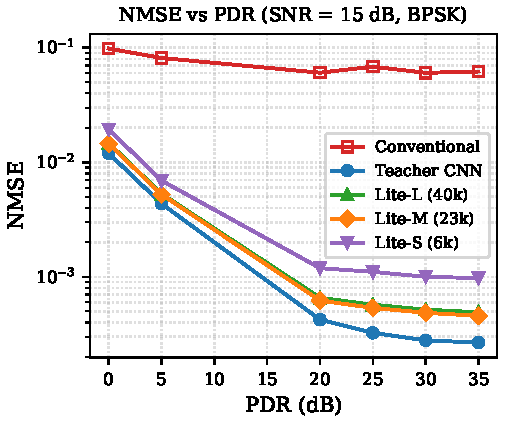
\includegraphics[width=\columnwidth]{nmse_vs_pdr.pdf}
    \caption{NMSE vs.\ PDR at SNR = 15\,dB, BPSK. All distilled students substantially outperform the conventional estimator.}
    \label{fig:nmse_pdr}
\end{figure}

\begin{figure}[t]
    \centering
    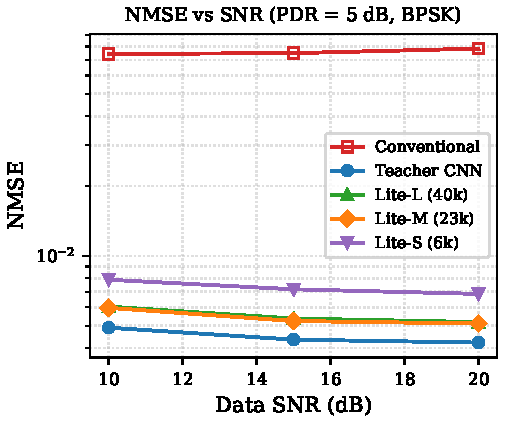
\includegraphics[width=\columnwidth]{nmse_vs_snr.pdf}
    \caption{NMSE vs.\ data SNR at PDR = 5\,dB, BPSK. Performance ordering is consistent across the SNR range.}
    \label{fig:nmse_snr}
\end{figure}

\subsection{BER Performance}

Fig.~\ref{fig:ber_pdr} presents BER versus PDR at SNR = 18\,dB with BPSK and LMMSE detection. At the moderate operating point of PDR = 5\,dB, Lite-M achieves a BER of $4.90 \times 10^{-4}$, close to the teacher's $4.86 \times 10^{-4}$ and the perfect-CSI bound of $3.39 \times 10^{-4}$. The conventional estimator, in contrast, yields a BER of $6.23 \times 10^{-2}$, more than two orders of magnitude worse.

At the challenging high-PDR point of 20\,dB, Lite-M exhibits a BER of $2.68 \times 10^{-3}$ compared to the teacher's $1.23 \times 10^{-3}$, reflecting the expected difficulty of distillation in the high-interference regime. Lite-S shows further degradation at this operating point with a BER of $1.12 \times 10^{-2}$.

Fig.~\ref{fig:ber_snr} shows BER versus SNR at PDR = 5\,dB. At 18\,dB, Lite-M and Lite-L track the teacher tightly, with all three achieving BER below $5 \times 10^{-4}$.

\begin{figure}[t]
    \centering
    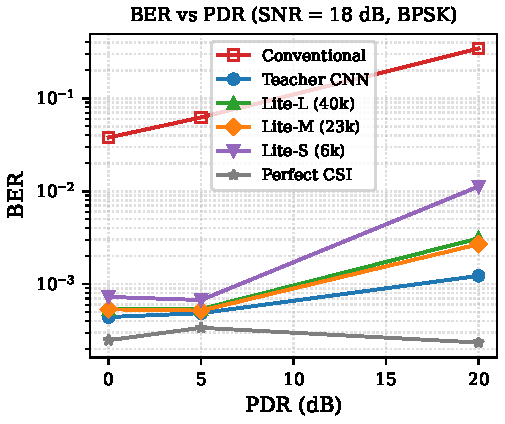
\includegraphics[width=\columnwidth]{ber_vs_pdr.pdf}
    \caption{BER vs.\ PDR at SNR = 18\,dB, BPSK, LMMSE detection.}
    \label{fig:ber_pdr}
\end{figure}

\begin{figure}[t]
    \centering
    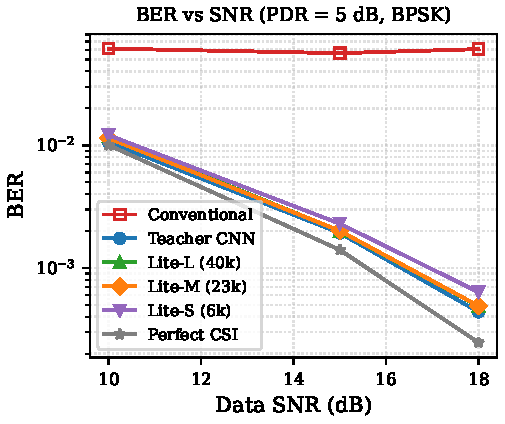
\includegraphics[width=\columnwidth]{ber_vs_snr.pdf}
    \caption{BER vs.\ data SNR at PDR = 5\,dB, BPSK, LMMSE detection.}
    \label{fig:ber_snr}
\end{figure}

\subsection{Accuracy-Efficiency Tradeoff}

Fig.~\ref{fig:tradeoff} plots NMSE against parameter count, illustrating the Pareto frontier. Lite-M represents the best tradeoff point: it provides a $10.8\times$ parameter reduction with only a modest NMSE increase. Lite-L offers slightly better accuracy for a smaller compression factor, while Lite-S provides extreme compression at the cost of more noticeable degradation.

\begin{figure}[t]
    \centering
    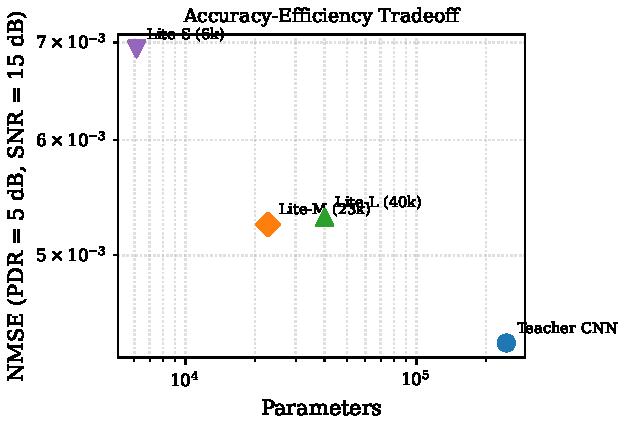
\includegraphics[width=\columnwidth]{tradeoff.pdf}
    \caption{Accuracy-efficiency tradeoff. Lite-M provides the best balance of compression and estimation quality.}
    \label{fig:tradeoff}
\end{figure}

% ══════════════════════════════════════════════════════════════
\section{Complexity and Efficiency Analysis}
\label{sec:complexity}

Table~\ref{tab:complexity} summarizes the model complexity and measured inference latency. The teacher has 245,473 parameters and requires 3.20\,ms per inference. All three student models achieve substantial parameter reductions: $6.1\times$ for Lite-L, $10.8\times$ for Lite-M, and $40.0\times$ for Lite-S.

Measured latency speedups range from $1.9\times$ to $2.1\times$, substantially smaller than the parameter reduction ratios. Notably, the latency ordering across students is not strictly monotonic with parameter count: Lite-S (6k params) and Lite-L (40k params) both measure approximately 1.52\,ms, while Lite-M (23k params) measures 1.68\,ms. This reflects the MPS backend's kernel dispatch overhead and memory-bandwidth characteristics, which dominate over pure arithmetic cost for these small models. Speedup ratios may differ on other hardware platforms (e.g., mobile NPUs, embedded GPUs) where compute-bound execution is more likely.

\begin{table}[t]
\centering
\caption{Model complexity comparison. Latency measured on Apple MPS with batch size 1, averaged over 50 iterations.}
\label{tab:complexity}
\begin{tabular}{lrrr}
\toprule
Model & Params & Latency (ms) & Speedup \\
\midrule
Teacher CNN & 245,473 & 3.20 & 1.00$\times$ \\
Lite-L & 40,049 & 1.52 & 2.10$\times$ \\
Lite-M & 22,789 & 1.68 & 1.91$\times$ \\
Lite-S & 6,137 & 1.52 & 2.11$\times$ \\
\bottomrule
\end{tabular}
\end{table}


Table~\ref{tab:operating_points} compares all methods at a representative operating point (PDR = 5\,dB). Lite-M achieves NMSE of $5.25 \times 10^{-3}$ and BER of $4.90 \times 10^{-4}$ with only 22,789 parameters, representing a strong accuracy-efficiency tradeoff suitable for resource-constrained deployment.

\begin{table}[t]
\centering
\caption{Key operating-point comparison at PDR = 5\,dB. NMSE at SNR = 15\,dB; BER at SNR = 18\,dB with BPSK.}
\label{tab:operating_points}
\begin{tabular}{lrll}
\toprule
Method & Params & NMSE & BER \\
\midrule
Conventional & --- & 8.1410e-02 & 6.0666e-02 \\
Teacher CNN & 245,473 & 4.3520e-03 & 4.3899e-04 \\
Lite-L & 40,049 & 5.3068e-03 & 4.8803e-04 \\
Lite-M & 22,789 & 5.2490e-03 & 4.9049e-04 \\
Lite-S & 6,137 & 6.9299e-03 & 6.3518e-04 \\
Perfect CSI & --- & --- & 2.4647e-04 \\
\bottomrule
\end{tabular}
\end{table}


% ══════════════════════════════════════════════════════════════
\section{Conclusion}
\label{sec:conclusion}

We have presented a knowledge distillation approach for compressing the CNN-aided channel estimator in the Zak-OTFS superimposed spread pilot framework. Our proposed Lite-M student model achieves a $10.8\times$ parameter reduction (from 245k to 23k) with NMSE within 0.9\,dB of the teacher and comparable BER at moderate PDR values. The Lite-L variant provides a higher-fidelity option with $6.1\times$ compression, while Lite-S demonstrates the limits of aggressive compression at $40\times$ reduction.

We emphasize that our results characterize an accuracy-efficiency tradeoff rather than claiming universal superiority over the teacher. The distilled students are most effective at moderate PDR values (5--10\,dB), where the teacher itself performs well. At high PDR, the gap widens as expected.

Our implementation includes a complete baseline reimplementation (no official code accompanies~\cite{zakotfs2024}) together with all distillation training, evaluation, and benchmarking infrastructure. A public code release is planned. Future work includes feature-based distillation, quantization-aware training, and evaluation on hardware platforms where latency scales proportionally with compute.

% ══════════════════════════════════════════════════════════════
\bibliographystyle{IEEEtran}
\bibliography{references}

\end{document}
